%!TeX root=../tese.tex
%("dica" para o editor de texto: este arquivo é parte de um documento maior)

\chapter{O painel administrativo}
\label{cap:implementacao}

Este capítulo descreve a implementação do painel administrativo desenvolvido para apoiar o piloto BikeSP. A Seção~\ref{sec:arquitetura} apresenta a arquitetura de software do sistema completo, mostrando como o painel se integra aos demais componentes. A Seção~\ref{sec:processo-desenvolvimento} descreve o processo de desenvolvimento adotado pela equipe. A Seção~\ref{sec:abas-painel} detalha cada uma das funcionalidades implementadas nas diferentes abas do painel, incluindo inserção de usuários, gerenciamento de coortes, bônus, remuneração, contestações, viagens, notificações e localizações.

\section{Arquitetura de software}
\label{sec:arquitetura}
O sistema BikeSP é composto por múltiplos componentes distribuídos em diferentes
infraestruturas, conforme ilustrado na Figura~\ref{fig:arquitetura}. O
\textbf{Painel Administrativo} atua como componente central de orquestração,
integrando-se aos demais módulos do sistema.

Os usuários realizavam inscrição através do \textbf{Formulário LimeSurvey}, hospedado em uma máquina virtual NuvemUSP. Após
o período de inscrições, um administrador utiliza o painel para executar um
\emph{script} que extraía os dados dos candidatos do LimeSurvey e os inseria no
banco de dados PostgreSQL do BikeSP, já filtrando os candidatos selecionados pela 
equipe de pesquisa pelos critérios de elegibilidade e balanceamento experimental definidos.

A máquina virtual Amazon hospeda o
\textbf{Banco de Dados PostgreSQL} e o \textbf{Back-end Flask}, que implementa a
lógica de negócio do sistema (validação de viagens, cálculo de créditos,
gerenciamento de usuários e coortes). O painel comunica-se com o back-end via
APIs REST para consultar e manipular dados.

O \textbf{App Android} é utilizado pelos participantes
para registrar viagens de bicicleta. As viagens são enviadas ao back-end, que as
valida e processa. O painel permite que administradores visualizem, auditem e, se
necessário, corrijam dados de viagens (por exemplo, erros de geolocalização).

O sistema integra-se com: (i) \textbf{Google
Firebase} para autenticação e notificações push; (ii) \textbf{APIs de
Geolocalização} (TomTom e Nominatim) para validação e correção de coordenadas
GPS; e (iii) \textbf{Loja Virtual SPTrans} para processamento de pagamentos dos
créditos acumulados pelos participantes.

O painel é acessado pela \textbf{equipe de suporte} e
operação, permitindo gestão de cadastros, atribuição de coortes, criação de
bônus, aprovação de contestações e geração de relatórios para a equipe de
economistas.

\begin{figure}[htb]
  \centering
  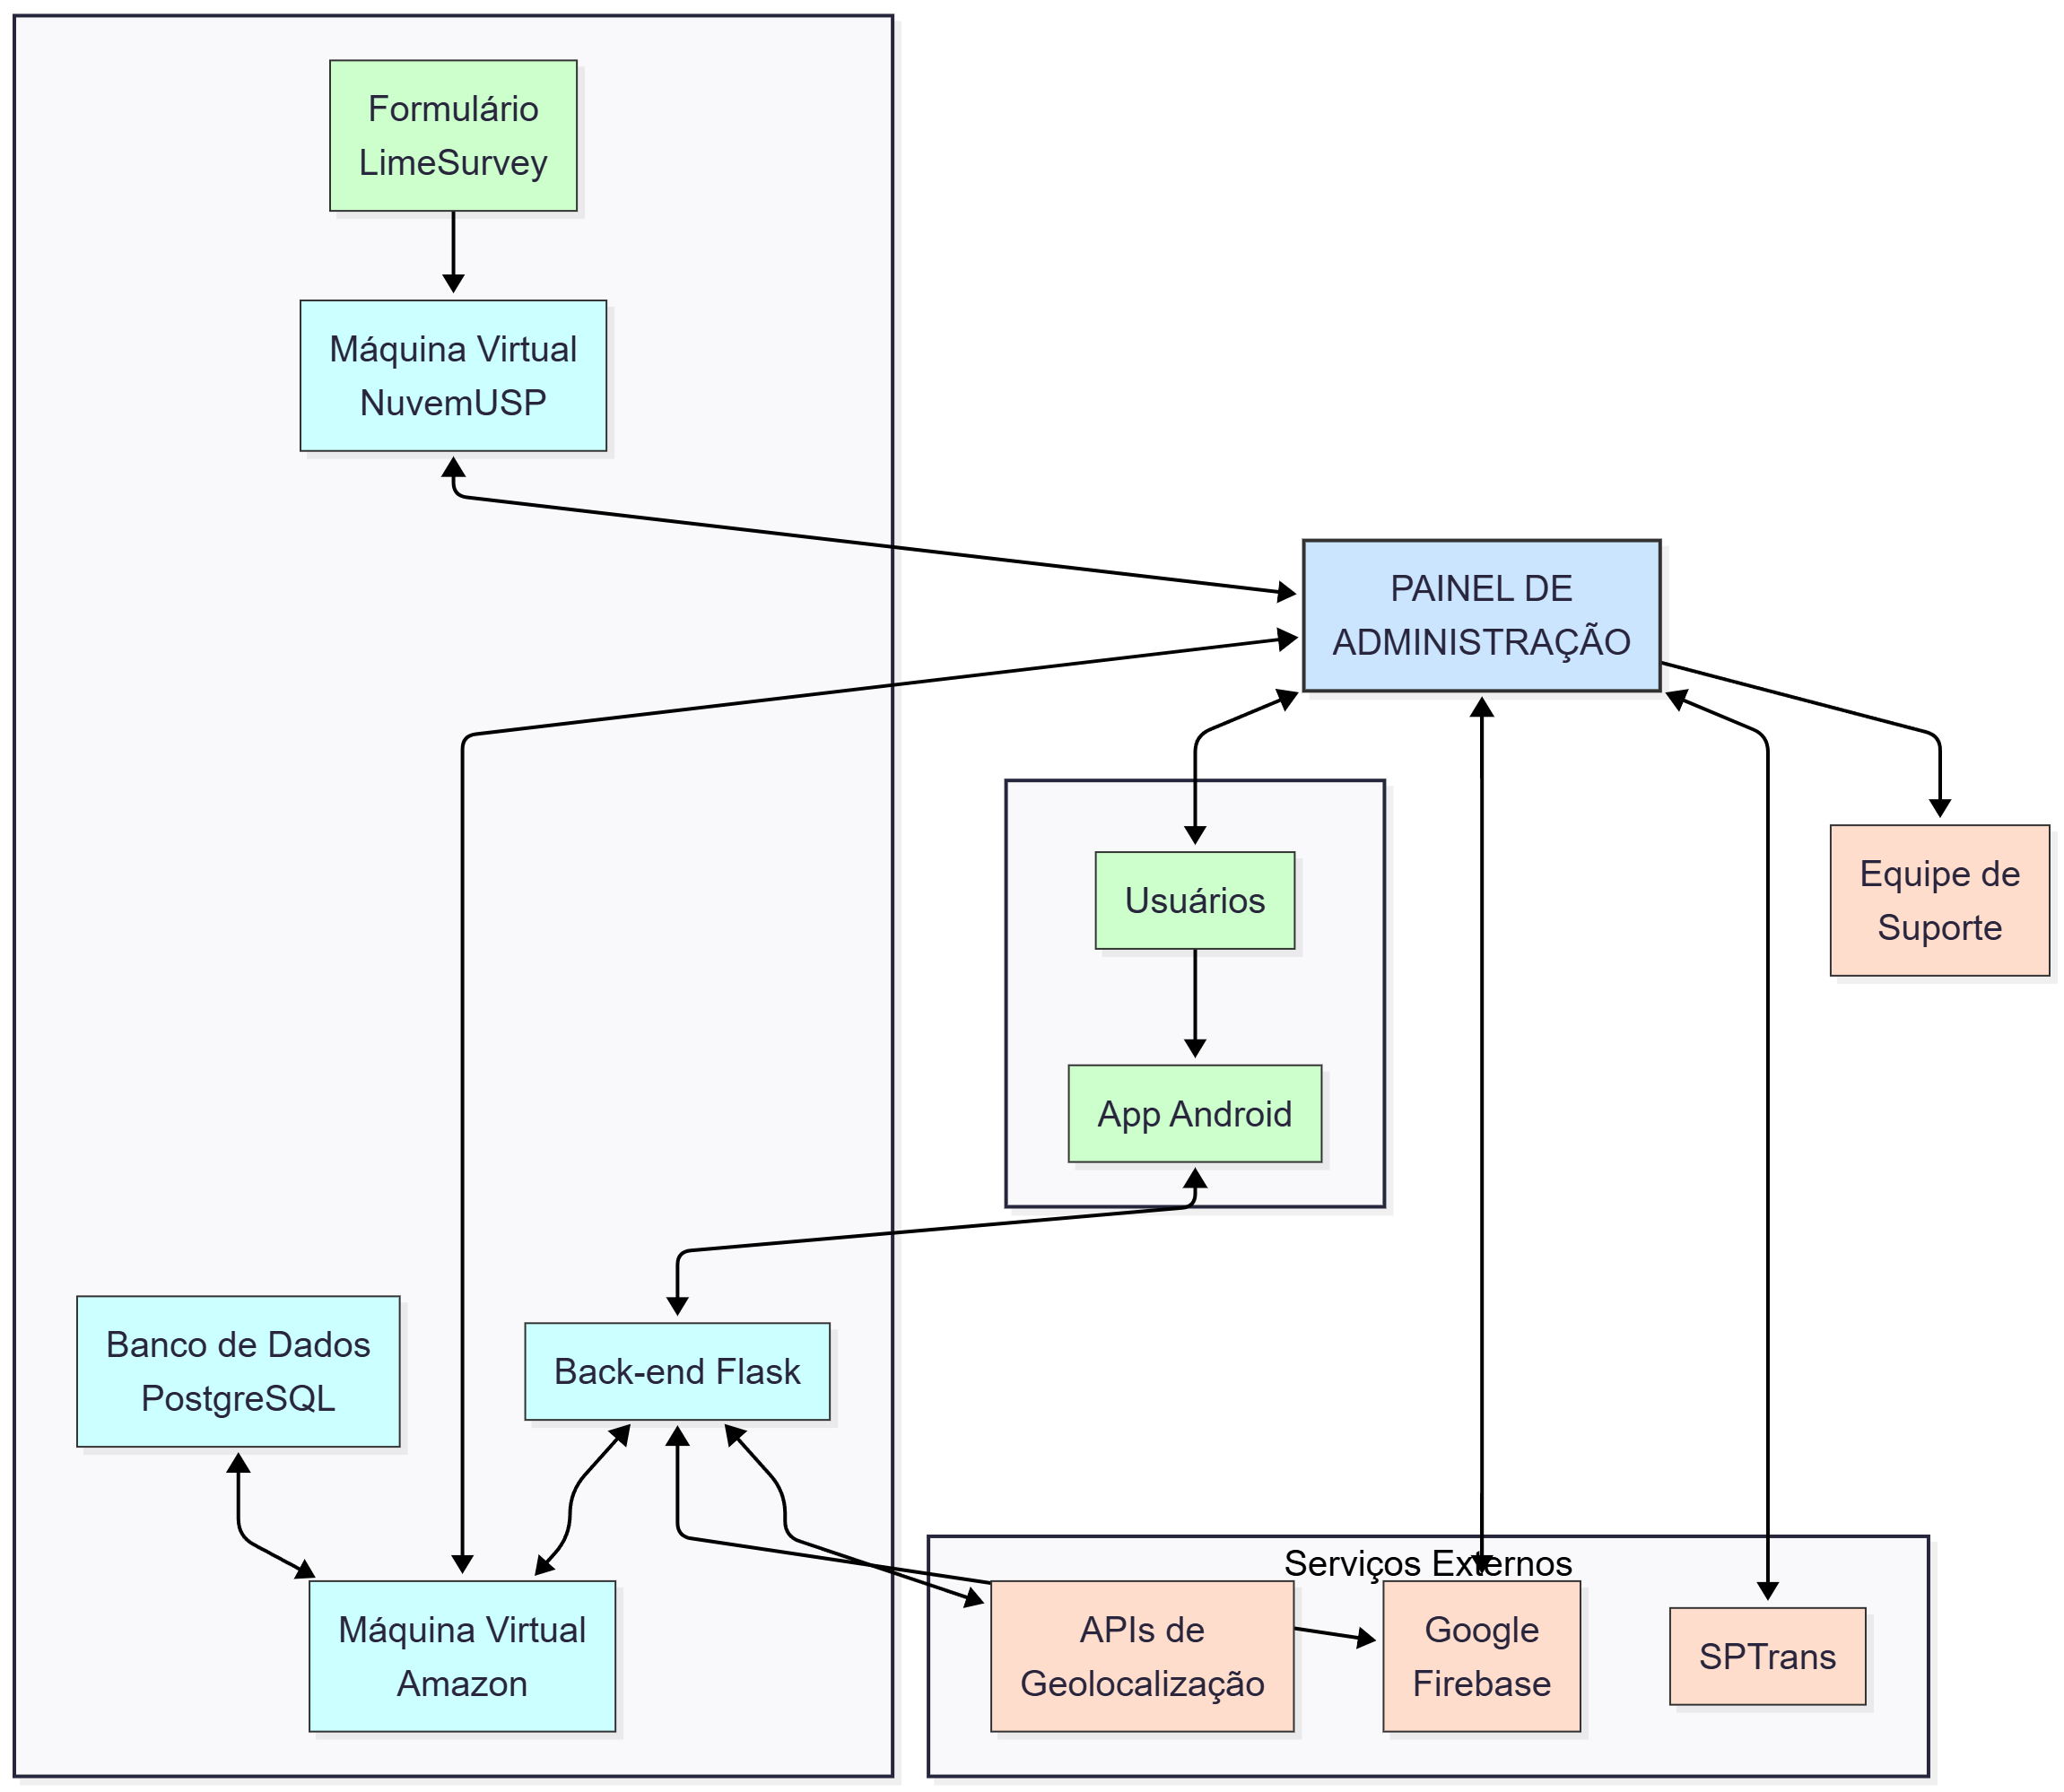
\includegraphics[width=0.95\textwidth]{diagrama_3.png}
  \caption{Diagrama simplificado dos componentes do sistema BikeSP.}
  \label{fig:arquitetura}
\end{figure}

\section{Processo de desenvolvimento}
\label{sec:processo-desenvolvimento}
O desenvolvimento envolveu múltiplos stakeholders e ciclos curtos de validação:
economistas (por exemplo, Thainá), suporte/atendimento (Sávio), coordenação e
orientação (Fábio e Paulo), além da equipe técnica. As demandas foram
priorizadas e acompanhadas via registro de \textit{issues}, criação de
\textit{pull requests} e revisão colaborativa, organizada no Gitlab, com homologação contínua durante
o pré-teste, o período de inscrições, a preparação de julho e a execução do
piloto.

\section{Abas do painel e uso no piloto}
\label{sec:abas-painel}

\subsection{Inserção de usuários}
%!TeX root=../tese.tex
%("dica" para o editor de texto: este arquivo é parte de um documento maior)

% Conteúdo da subseção sobre Inserção de Usuários
% Este arquivo é importado em 02-implementacao.tex

\textbf{Fluxo de inscrição e coleta de dados iniciais.} O processo de recrutamento de participantes para o piloto BikeSP iniciou-se com ampla divulgação midiática (entrevistas em jornais, redes sociais, site institucional), direcionando interessados para formulário online hospedado em instância LimeSurvey na NuvemUSP. O formulário coletava: dados pessoais (nome, CPF, email, data de nascimento, gênero), número do Bilhete Único (pré-requisito para participação, pois remuneração seria creditada neste cartão), senha para acesso ao aplicativo móvel, endereços textuais de até três localizações (tipicamente casa e trabalho/escola), telefone para contato, e concordância com Termo de Consentimento Livre e Esclarecido (TCLE --- documento obrigatório aprovado por Comitê de Ética para pesquisas envolvendo seres humanos). Durante o período de inscrições, o formulário recebeu aproximadamente 3.000 submissões, volume que requeria automação para transferência ao banco de dados PostgreSQL do sistema BikeSP.

\textbf{Script de inserção automatizada.} A funcionalidade de inserção em lote, acessível via botão ``Inserir Usuários!'' no painel administrativo, executa script que: (i) conecta à API do LimeSurvey e baixa todas respostas ainda não processadas; (ii) itera sobre cada resposta aplicando validações (CPF válido via algoritmo de verificação de dígitos, email em formato correto e único no sistema, Bilhete Único com 15 dígitos numéricos, senha com mínimo de caracteres configurável); (iii) criptografa a senha antes de armazenar (segurança crítica); (iv) geocodifica endereços textuais chamando APIs externas (TomTom, Google Maps, Nominatim OSM) para converter em coordenadas GPS; (v) armazena dados cadastrais da pessoa, vinculação do cartão Bilhete Único com status ativo, e coordenadas de casa e trabalho; (vi) atribui participante a coorte inicial (pode ser randomizado ou seguir configuração padrão); e (vii) registra logs detalhados de sucesso/falha para cada usuário processado.

Execução ocorre em thread separada (processamento assíncrono) para não bloquear interface administrativa durante operação (geocodificação via APIs externas é gargalo principal). Botão fica desabilitado durante processamento, prevenindo cliques duplos que iniciariam múltiplas execuções simultâneas. Mensagem inicial ``Usuários novos estão sendo inseridos!'' confirma início; mensagem final reporta quantidade inserida (``X usuários inseridos com sucesso'') ou erros encontrados.

\begin{figure}[H]
  \centering
  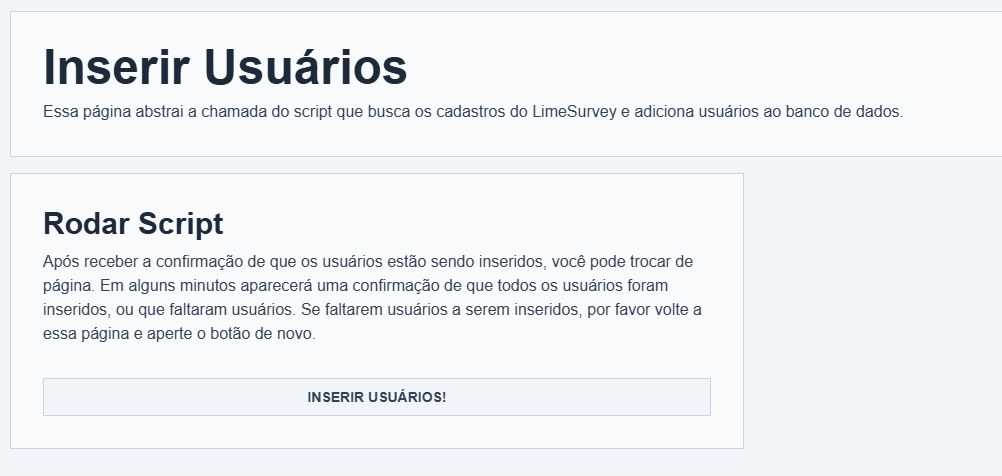
\includegraphics[width=0.95\textwidth]{figuras/inserir_usuarios.PNG}
  \caption{Interface de inserção de usuários no painel administrativo, com botão para executar o script de importação do LimeSurvey.}
  \label{fig:insercao_usuarios}
\end{figure}

\textbf{Tratamento de falhas e idempotência.} Sistema implementa verificação de CPF existente antes de tentar inserção, prevenindo duplicações mesmo se script executado múltiplas vezes sobre mesmas respostas do LimeSurvey (comportamento idempotente). Quando endereço falha em geocodificação (10-20\% dos casos conforme discussão na subseção de Localizações), localização é criada marcada como ``inválida'', permitindo participante existir no sistema mas impedindo uso daquela localização em viagens até correção manual via interface administrativa. Esta estratégia parcialmente otimista (criar usuário mesmo com dados incompletos) prioriza não bloquear participação --- melhor ter usuário com localização a corrigir que rejeitar inscrição completamente. Mensagens de aviso (``Y usuários faltaram a serem inseridos'', ``Z endereços não puderam ser geocodificados'') orientam reexecução do script (para tentar novamente usuários que falharam transientemente) e correção manual de localizações.

\textbf{Critérios de elegibilidade e seleção.} Embora formulário LimeSurvey coletasse ~3.000 inscrições, apenas 1.217 participantes foram efetivamente inseridos no sistema e incluídos no piloto. Critérios de elegibilidade aplicados durante seleção (manualmente por economistas antes de liberar CPFs para script de inserção) incluíam: residência em São Paulo (verificação via CEP), posse de Bilhete Único ativo, não ser cicloativista regular (auto-declaração --- para evitar viés de seleção, experimento buscava medir impacto em usuários representativos, não entusiastas pré-dispostos), e disponibilidade para participar durante seis meses. Preferência adicional para diversidade de perfis socioeconômicos e geográficos. Esta separação entre coleta ampla pelo LimeSurvey e inserção seletiva pelo script permitiu flexibilidade experimental mantendo integridade metodológica.

\textbf{Sincronização com atribuição de coortes.} Primeira execução do script, inserindo ~1.200 usuários simultaneamente, foi coordenada com atribuição inicial de coortes via funcionalidade de upload em lote (descrita na subseção de Coortes). Workflow combinado: economistas geravam CSV com (CPF, ID\_Coorte) aplicando randomização estratificada; administrador executava script de inserção LimeSurvey→PostgreSQL; aguardava confirmação de sucesso; imediatamente executava upload de atribuição de coortes; verificava balanceamento (~400 usuários por coorte); enviava notificações de boas-vindas via sistema de notificações. Este processo único e crítico ocorreu na véspera do início oficial do piloto, requirendo coordenação temporal precisa para permitir resolução de problemas antes que participantes recebessem instruções para ativar o aplicativo.

\textbf{Funcionalidade específica para o piloto.} Este processo de inserção em lote via script administrativo foi desenvolvido exclusivamente para o projeto piloto, onde era necessário selecionar manualmente 1.217 participantes dentre 3.000 inscritos aplicando critérios de elegibilidade (residência em São Paulo, não ser cicloativista, diversidade socioeconômica). O formulário LimeSurvey serviu como porta de entrada ampla para candidatos, enquanto o script de inserção permitia controle fino sobre quem seria efetivamente incluído no experimento controlado.

Para a implementação municipal em larga escala (~10.000-50.000 usuários), quando o programa BikeSP for liberado para todos os ciclistas de São Paulo, esta arquitetura de duas etapas (LimeSurvey → script → banco de dados) seria substituída por cadastro direto e automático via aplicativo móvel. Usuários interessados instalariam o aplicativo, preencheriam dados cadastrais diretamente na interface, e seriam automaticamente integrados ao sistema sem necessidade de aprovação ou processamento em lote por administradores. O formulário LimeSurvey e o script de inserção foram ferramentas necessárias apenas para o contexto experimental do piloto, não fazendo parte da arquitetura planejada para a política pública permanente.




\subsection{Usuários}
%!TeX root=../tese.tex
%("dica" para o editor de texto: este arquivo é parte de um documento maior)

% Conteúdo da subseção sobre Usuários
% Este arquivo é importado em 02-implementacao.tex

Durante o piloto BikeSP, com
aproximadamente 1.200 participantes selecionados dentre 3.000 inscritos, a equipe de
suporte enfrentava demandas diárias de atendimento. Questões como ``não consigo acessar o aplicativo'', ``minha viagem não foi
computada'', ``como altero meu endereço cadastrado'' requeriam identificação rápida
do participante no sistema para diagnóstico e resolução. A interface de gerenciamento
de usuários tornou-se, portanto, o
ponto de partida no sistema administrativo  para praticamente todas as operações de suporte,
auditoria e análise.

A tela de usuários apresenta
tabela com seis colunas principais: ID (identificador único), nome
completo, email, CPF, número do Bilhete Único, e indicador mostrando se o participante
completou o cadastro de senha (permitindo acesso ao aplicativo). O sistema consulta dados pessoais vinculados aos cartões Bilhete Único ativos, utilizando técnicas de otimização para obter contagem total sem sobrecarregar o banco de dados --- importante para responsividade em conjuntos de dados com milhares de registros. A coluna ``Tem Senha'' verifica se existe senha cadastrada para aquele usuário, indicador crucial para diagnosticar
problemas de acesso (usuário inscrito mas sem senha configurada não consegue entrar no aplicativo).

O sistema oferece busca unificada por nome
(parcial, \textit{case-insensitive}\@) ou ID exato.
Por exemplo, buscar ``silva'' retorna ``Silva João'', ``Silvana Costa'', ``Marcos da
Silva'', enquanto buscar ``123'' retorna apenas o participante com ID exatamente 123.
Esta abordagem dual (nome parcial vs. ID exato) equilibra flexibilidade para buscas
exploratórias (quando administrador conhece apenas nome aproximado) e precisão para
operações dirigidas (quando ID já foi identificado em interação anterior ou viagem
específica). Importante notar que a busca não cobre email, CPF ou Bilhete
Único diretamente; para localizar por estes atributos, utiliza-se ordenação combinada com inspeção visual. A Figura~\ref{fig:usuarios_listagem} apresenta a interface de listagem (dados fictícios para fins ilustrativos).


\begin{figure}[htb]
    \centering
    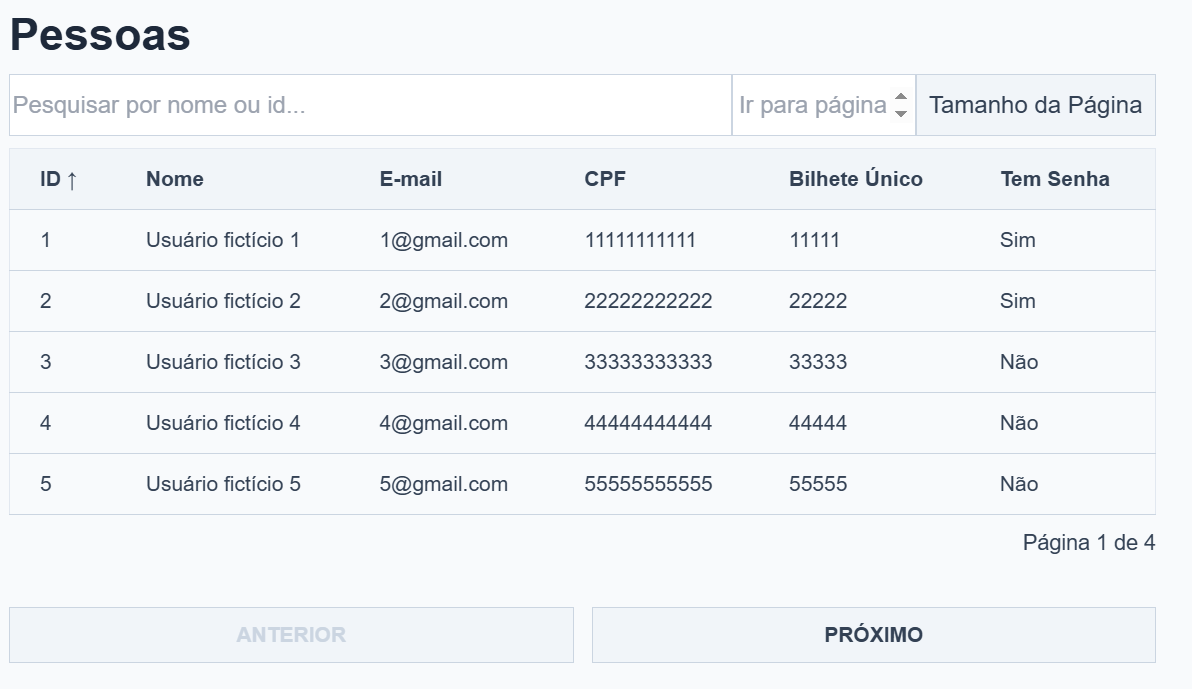
\includegraphics[width=0.95\textwidth]{figuras/pessoas.PNG}
    \caption{Interface de listagem de usuários com funcionalidades de busca, ordenação e paginação (dados fictícios).}
    \label{fig:usuarios_listagem}
  \end{figure}

Cada cabeçalho de coluna funciona como botão de
ordenação: primeiro clique ordena ascendentemente, segundo clique inverte para
descendente, com indicadores visuais (setas ↑↓) mostrando coluna ativa e direção.
Ordenação por nome facilita localização alfabética; por ID permite identificar
usuários cadastrados cronologicamente (IDs crescentes); por ``Tem Senha'' agrupa
participantes que completaram vs. não completaram ativação.

A interface oferece quatro densidades: 5, 10, 15
(padrão) ou 20 usuários por página, selecionáveis via dropdown. Navegação ocorre por
botões ``Anterior''/``Próximo'' (desabilitados nos extremos) ou campo de entrada
direta ``Ir para página X'', validando automaticamente se página solicitada existe.
Indicador ``Página X de Y'' fornece senso de escala do conjunto de dados. Esta
flexibilidade mostrou-se útil em diferentes contextos operacionais: densidade baixa
(5-10 itens) para inspeção cuidadosa com múltiplas abas abertas; densidade alta
(20 itens) para varredura rápida ou busca semi-manual quando termo de busca textual
não é aplicável.

A tela de usuários serve como ponto de
entrada para diversos fluxos operacionais críticos durante o piloto. \textit{Cenário
1: Suporte via email} --- participante reporta viagem não creditada; administrador
busca por nome, identifica ID, navega à tela de viagens filtrando por aquele ID,
localiza viagem em questão e diagnostica problema (ex: trajeto fora dos locais
cadastrados). \textit{Cenário 2: Problema de acesso ao app} --- participante não
consegue fazer login; administrador busca por nome, verifica coluna ``Tem Senha''; se
``Não'', orienta participante a completar cadastro via funcionalidade de redefinição
de senha. \textit{Cenário 3: Ajuste de localização} --- participante mudou de
endereço; administrador identifica ID, navega à tela de localizações, atualiza
coordenadas e endereço textual. \textit{Cenário 4: Contestação de viagem} ---
administrador recebe disputa; identifica usuário, obtém ID, acessa tela de
contestações para processar aprovação/rejeição. Em todos estes cenários, a rapidez
da busca e clareza da informação apresentada determinam eficiência do atendimento.

Durante o período de piloto, a
tela de usuários foi acessada diariamente pela equipe de suporte.
A métrica ``Tem Senha'' permitiu identificar participantes que não completaram ativação do aplicativo, 
orientando campanhas de engajamento. Recursos como ordenação e paginação reduziram significativamente a 
dependência de consultas manuais ao banco de dados, tornando as operações de suporte de primeiro nível mais ágeis
e acessíveis para toda a equipe.



\subsection{Coortes}
\label{sec:coortes}
%!TeX root=../tese.tex
%("dica" para o editor de texto: este arquivo é parte de um documento maior)

% Conteúdo da subseção sobre Coortes
% Este arquivo é importado em 02-implementacao.tex

O piloto BikeSP foi estruturado como experimento controlado randomizado (RCT --- \textit{Randomized Controlled Trial}) visando responder questão de implementação fundamental (IQ1): ``Como o número de viagens de bicicleta varia com diferentes valores de remuneração?'' Esta metodologia permite isolar efeito de incentivos financeiros de fatores confundidores, fornecendo evidências causais robustas para regulamentação da Lei Municipal 16.547/2016. Participantes foram alocados a três coortes (grupos experimentais) com diferentes níveis de remuneração por quilômetro pedalado: Coorte 0 (controle, sem remuneração), Coorte 1 (incentivo baixo, R\$~0,30/km, equivalente a 1/16 da tarifa de transporte público), e Coorte 2 (incentivo alto, R\$~0,60/km, equivalente a 1/8 da tarifa). A escolha destes valores baseou-se em estudo do Banco Mundial sobre elasticidade-preço de demanda por ciclismo em São Paulo, onde remunerações nesta faixa mostraram impacto significativo sem comprometer viabilidade orçamentária.

Característica distintiva do desenho foi rotação semanal de coortes: cada participante alternava entre as três condições a cada semana, experimentando todas coortes ao longo do piloto. Esta estratégia reduz viés de seleção (todos expostos a todas condições) e aumenta poder estatístico para detectar diferenças intra-indivíduos (cada participante serve como próprio controle). Adicionalmente, remuneração foi desativada em finais de semana para todas coortes, permitindo observar retenção de comportamento na ausência de incentivo financeiro --- descoberta notável foi que 9 das 10 viagens mais longas ocorreram justamente nestes períodos sem remuneração, evidência de internalização do hábito de pedalar.

A interface de coortes oferece funcionalidades para criação, listagem, e atribuição de participantes a grupos. Criação/atualização requer ID numérico único (1, 2, 3) e valor de remuneração por quilômetro; sistema automaticamente cria nova coorte se ID inexistente, ou atualiza valor se ID já cadastrado (útil para ajustes durante piloto sem recriar grupo). Listagem exibe ID, remuneração formatada como moeda (R\$~0,30), e quantidade de membros associados, com busca por ID específico e paginação (5 itens/página). Durante piloto com 1.217 participantes, distribuição manteve-se aproximadamente balanceada: ~400 participantes por coorte em qualquer semana dada, essencial para comparabilidade estatística.


 \begin{figure}[H]
   \centering
   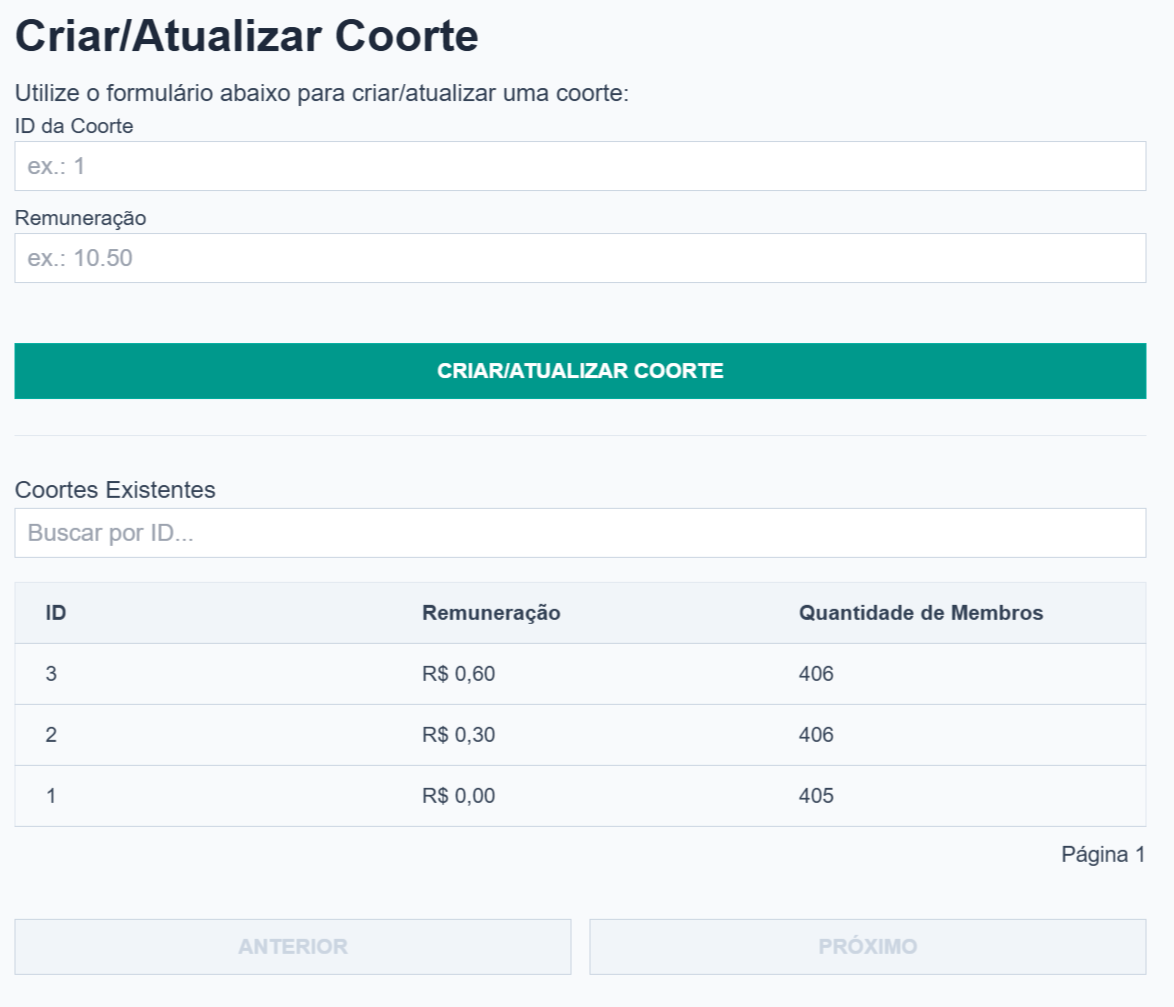
\includegraphics[width=0.95\textwidth]{figuras/coortes.PNG}
   \caption{Interface de gerenciamento de coortes e visualização de quantidade de participantes por grupo.}
   \label{fig:coortes_listagem}
 \end{figure}

 A tela dedicada lista todos usuários com respectivas coortes, exibindo ID, nome, email, total de viagens realizadas, e ID da coorte atual. Sistema de filtros combinados permite: busca por ID de pessoa, nome parcial (\textit{case-insensitive}), email, ID de coorte específica, e intervalo de viagens (mínimo/máximo). Filtros aplicam-se simultaneamente via lógica AND e persistem durante paginação. Esta funcionalidade atendeu múltiplos casos de uso: (i) verificar balanceamento de grupos (filtrar por ID de coorte, observar contagem); (ii) identificar participantes inativos (por exemplo, buscando com o filtro de usuários com no máximo 2 viagens); (iii) selecionar participantes altamente engajados para entrevistas qualitativas (por exemplo, buscando com o filtro de usuários com no mínimo 30 viagens); (iv) auditar atribuições após rotação semanal (exportar CSV, comparar com planilha esperada).

 \begin{figure}[H]
    \centering
    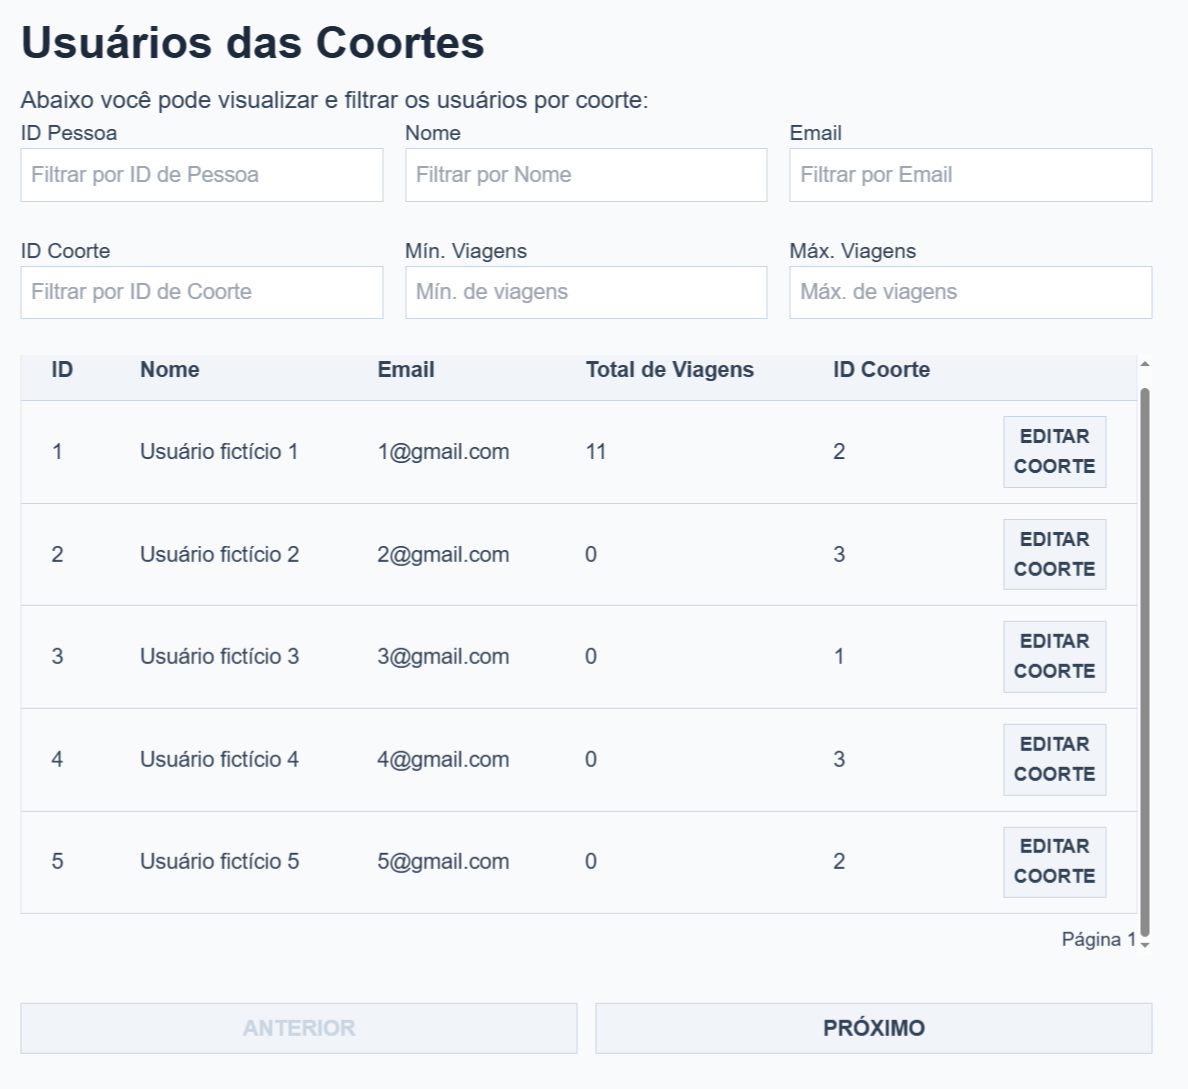
\includegraphics[width=0.95\textwidth]{figuras/usuario_coortes_zoom.PNG}
    \caption{Interface de filtragem de participantes por coorte.}
    \label{fig:coortes_listagem_usuarios}
  \end{figure}

Para correções pontuais, administrador pode editar coorte de usuário específico clicando ``Editar Coorte'' na linha da tabela, alterando ID para nova coorte ou deixando vazio para remover atribuição. Para operações em massa (rotação semanal), funcionalidade de upload via CSV permite atribuições em lote: arquivo com duas colunas (CPF;ID\_Coorte) separadas por ponto-e-vírgula, sem cabeçalho, codificação UTF-8. Sistema valida linha por linha antes de processar: CPF deve existir, coorte destino deve estar cadastrada, CPFs não podem duplicar. Erros específicos (``CPF 12345678901 não encontrado'', ``Coorte 99 não existe'') facilitam correção e reupload. Processamento atômico garante que ou todas atribuições são aplicadas ou nenhuma, prevenindo estados parciais que comprometeriam integridade experimental.

Durante piloto, rotação semanal típica seguia workflow: economistas geravam CSV com nova atribuição usando script (randomização estratificada por perfil socioeconômico e localização geográfica); administrador fazia upload via painel; sistema atualizava os registros; notificações push/email informavam participantes sobre nova remuneração vigente; exportação CSV pós-upload confirmava aplicação correta. Este processo de rotação semanal ao longo do projeto piloto evidenciou robustez e eficiência da funcionalidade.

\begin{figure}[H]
    \centering
    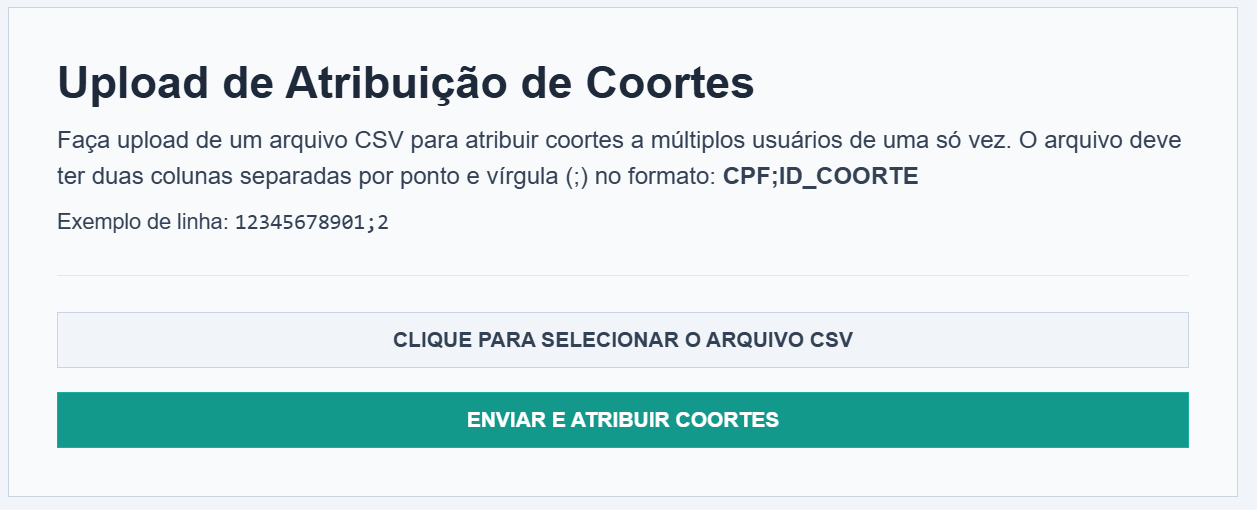
\includegraphics[width=0.95\textwidth]{figuras/upload_coortes.PNG}
    \caption{Interface de upload de atribuição de coortes em lote.}
    \label{fig:coortes_listagem_upload}
  \end{figure}

O botão de exportação gera CSV completo com ID, nome, CPF, email, ID da coorte, e valor de remuneração atual. O formato compatível com ferramentas estatísticas e facilita análises, o nome do arquivo gerado inclui a data da exportação, importante para criar um histórico versionado.

\begin{figure}[H]
    \centering
    
\includegraphics[width=0.95\textwidth]{figuras/exportar_coortes.PNG}
    \caption{Interface de exportação de coortes.}
    \label{fig:coortes_listagem_exportar}
  \end{figure}

O sistema implementa múltiplas salvaguardas: coortes não podem ser deletadas se possuem membros (previne perda acidental de atribuições); mudanças de remuneração em coorte ativa geram log detalhado (rastreabilidade de alterações durante experimento); tentativas de atribuir participante a coorte inexistente são rejeitadas (impossibilita referências órfãs); exportações registram timestamp e usuário que solicitou (auditoria de acesso a dados sensíveis).

A infraestrutura de gerenciamento de coortes no painel viabilizou análises sobre o impacto diferencial das remunerações. Os dados coletados durante o piloto permitirão investigar relações dose-resposta (comparando número de viagens entre diferentes valores de remuneração), validar a estratégia de rotação semanal, examinar retenção de participantes em cada coorte, e explorar heterogeneidade de efeitos por perfis socioeconômicos. Estas descobertas fundamentarão documento de recomendações para regulamentação da Lei Municipal 16.547/2016.





\subsection{Bônus}
\label{sec:bonus}
%!TeX root=../tese.tex
%("dica" para o editor de texto: este arquivo é parte de um documento maior)

% Conteúdo da subseção sobre Bônus
% Este arquivo é importado em 02-implementacao.tex

\textbf{Contexto e propósito dos bônus.} No contexto do piloto BikeSP, os bônus
representam uma ferramenta complementar de incentivo financeiro aos participantes,
independente das remunerações por quilômetro pedalado. Conforme planejado no desenho
do experimento, os bônus servem a múltiplos propósitos: (i) recompensar a conclusão
do curso gratuito ``Pedale com Segurança'' oferecido pelo Centro de Treinamento e
Educação de Trânsito (CETET) da CET; (ii) incentivar o preenchimento dos
questionários qualitativos aplicados em três momentos do piloto, garantindo maior
taxa de resposta e riqueza de dados; (iii) permitir ajustes administrativos e
correções pontuais de pagamento quando necessário; e (iv) viabilizar eventuais
campanhas promocionais temporárias para estimular a participação em momentos
estratégicos do experimento.

\textbf{Implementação técnica.} O painel administrativo oferece três
funcionalidades principais relacionadas a bônus: criação de novos tipos de bônus,
atribuição de bônus a usuários, e visualização e gerenciamento dos bônus
cadastrados. A arquitetura do sistema foi projetada para oferecer flexibilidade e controle sobre os incentivos.

\textbf{Criação de bônus.} Administradores podem cadastrar novos tipos de bônus
informando nome único (identificador), valor em reais, descrição textual, período
de validade (datas de início e fim, opcionais), e dois flags de controle: se o
bônus deve ser ativado automaticamente após criação, e se será visível aos
usuários no aplicativo móvel. A distinção entre bônus ativos/inativos e
visíveis/invisíveis oferece grande flexibilidade: bônus inativos não podem ser
concedidos (útil para pausar temporariamente um incentivo), enquanto bônus
invisíveis, mesmo quando concedidos e gerando remuneração, não aparecem na
listagem do aplicativo do usuário (útil para ajustes administrativos discretos ou
correções pontuais).

 \begin{figure}[H]
   \centering
   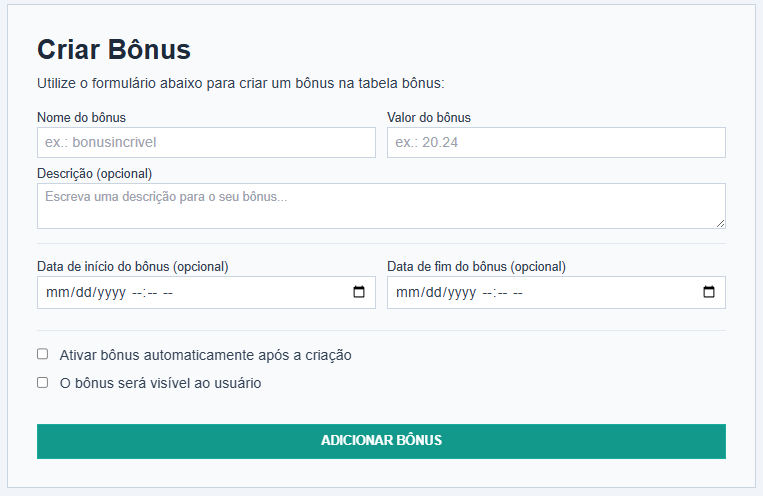
\includegraphics[width=0.95\textwidth]{figuras/criar_bonus.PNG}
   \caption{Formulário de criação de bônus no painel administrativo.}
   \label{fig:bonus_criar_form}
 \end{figure}

\textbf{Atribuição de bônus.} Para conceder um bônus a participantes, o
administrador informa os IDs dos usuários (separados por vírgula) e seleciona o
bônus desejado. O sistema valida diversas condições antes de processar a
concessão: o bônus deve estar ativo, não pode ter expirado (data de término não
ultrapassada), todos os usuários devem existir, e cada usuário pode receber cada
bônus apenas uma vez. Ao conceder um bônus com sucesso, o sistema não apenas registra a concessão, mas
também cria automaticamente uma remuneração correspondente ao valor do bônus e a
insere na fila de pagamentos (para posterior transferência aos cartões Bilhete
Único via Loja Virtual SPTrans). Caso algum usuário não atenda aos critérios, o
sistema reporta sucesso parcial, detalhando quantos usuários receberam o bônus e
quais apresentaram erros (por exemplo, ``5 sucesso(s), 2 erro(s): Usuário 101 já
possui este bônus; Usuário 203 não existe''). Esta funcionalidade de concessão em
lote reduz significativamente o tempo necessário para operações recorrentes, como
conceder o bônus do curso de segurança para todos os participantes que o
concluíram em determinada semana.

 \begin{figure}[H]
   \centering
   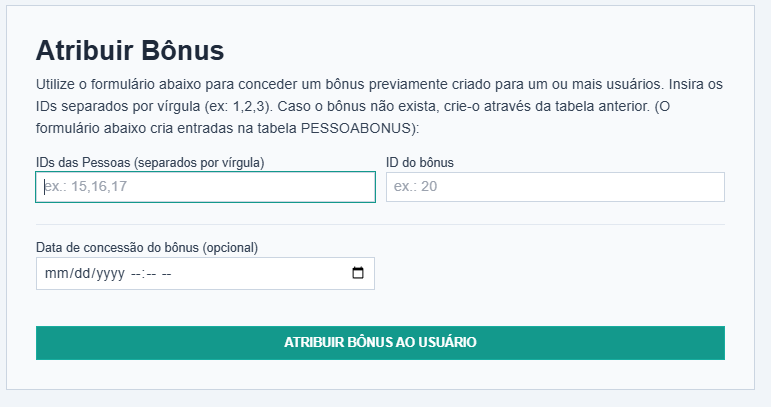
\includegraphics[width=0.95\textwidth]{figuras/atribuir_bonus.PNG}
   \caption{Formulário de atribuição de bônus aos participantes.}
   \label{fig:bonus_atribuir_form}
 \end{figure}

\textbf{Listagem e gerenciamento.} A tela de listagem exibe todos os bônus
cadastrados em formato tabular, apresentando ID, nome, valor, status de ativação,
visibilidade, descrição, período de validade e ações disponíveis. A interface
oferece busca por nome e paginação (5 itens por página). Cada linha da tabela
possui um botão para ativar ou desativar o bônus: bônus ativos exibem
botão vermelho ``Desativar'', enquanto bônus inativos exibem botão verde
``Ativar''. Importante notar que desativar um bônus não remove concessões já
realizadas nem afeta remunerações já geradas; apenas impede novas concessões
daquele tipo de bônus. Para facilitar a identificação dos IDs de usuários ao
atribuir bônus, a aba de bônus também oferece uma consulta integrada à tabela de
usuários, com busca por nome ou ID, ordenação por qualquer coluna e
paginação configurável da mesma forma que a tela de usuários.

\begin{figure}[H]
    \centering
    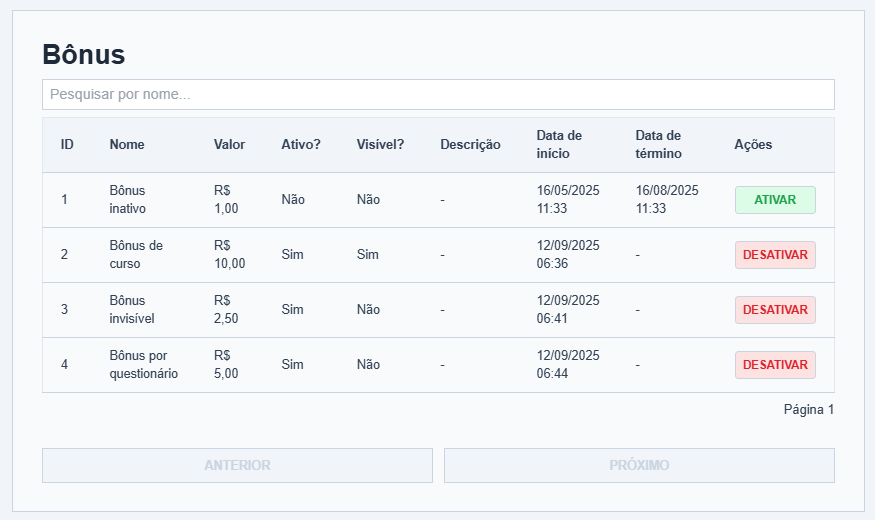
\includegraphics[width=0.95\textwidth]{figuras/bonus_listar.PNG}
    \caption{Listagem de bônus cadastrados com funcionalidades de busca, paginação e ativação/desativação.}
    \label{fig:bonus_listagem_form}
  \end{figure}
 

\textbf{Integração com o aplicativo móvel.} O aplicativo Android dos participantes
consome a API \texttt{POST /api/exibeBonus/} para listar os bônus concedidos ao
usuário autenticado. A API retorna apenas bônus marcados como visíveis, garantindo que ajustes administrativos invisíveis não
apareçam para os usuários finais. Esta separação entre visibilidade e concessão
oferece aos gestores do piloto a flexibilidade de realizar correções financeiras
sem necessariamente comunicá-las explicitamente aos participantes.

\textbf{Uso operacional no piloto.} Durante a execução do piloto, a
funcionalidade de bônus mostrou-se fundamental para diversos cenários operacionais:
concessão em lote do bônus do curso de segurança para centenas de participantes que
o concluíram simultaneamente; distribuição dos bônus dos questionários ao final de
cada período de coleta de dados qualitativos; correções pontuais quando erros de
geolocalização resultaram em viagens rejeitadas indevidamente (criando-se bônus
invisíveis de ajuste); A flexibilidade do sistema permitiu à
equipe operacional responder rapidamente a diferentes necessidades sem requerer
desenvolvimento de novas funcionalidades ou intervenções manuais no banco de dados.






\subsection{Remuneração}
\label{sec:remuneracao}
%!TeX root=../tese.tex
%("dica" para o editor de texto: este arquivo é parte de um documento maior)

% Conteúdo da subseção sobre Remuneração
% Este arquivo é importado em 02-implementacao.tex

A Lei Municipal 16.547/2016 estabeleceu
que o pagamento aos ciclistas do programa BikeSP seria realizado através de créditos
de transporte público, inseridos diretamente nos cartões Bilhete Único dos
participantes. Esta escolha reflete a intenção do governo municipal de integrar a
bicicleta ao sistema de transporte público, permitindo que os incentivos sejam
utilizados para deslocamentos multimodais (bicicleta + ônibus/metrô). O modelo de
remuneração por quilômetro pedalado, adotado também em iniciativas internacionais
como em Itajaí e na Holanda \citep{itajai2021, tennant2022}, visa recompensar a distância economizada ao
substituir outros modos de transporte, facilitando análises de impacto em poluição,
tráfego e saúde pública.

No desenho experimental do piloto, optou-se por valores de R\$~0,30 e R\$~0,60 por
quilômetro (equivalentes a 1/16 e 1/8 de uma passagem de transporte público,
respectivamente), com limite de duas viagens remuneradas por dia. Estes valores foram
baseados em estudo do Banco Mundial sobre disposição a pagar por ciclismo em São
Paulo \citep{worldbank2022}, que identificou que remunerações entre R\$~2,00 e R\$~3,00 por viagem
aumentavam em 38,4\% a probabilidade de escolher bicicleta sobre o modo atual,
efeito comparável à presença de ciclovias (43,4\%). A remuneração não foi
diferenciada por perfil de participante durante o piloto, pois um dos objetivos do
experimento era justamente compreender como o impacto da remuneração varia
segundo diferentes perfis demográficos e socioeconômicos.

O sistema de remuneração implementado no
painel administrativo gerencia três estados distintos do dinheiro: (i)
\texttt{aguardandoEnvio} --- valores de viagens aprovadas, bônus concedidos e
contestações deferidas que ainda não foram enviados à SPTrans; (ii)
\texttt{aguardandoResposta} --- valores já enviados à SPTrans através de arquivo
CSV, aguardando confirmação de creditação; e (iii) \texttt{concedido} --- valores
confirmados pela SPTrans como efetivamente creditados nos cartões Bilhete Único dos
participantes. Esta separação em estados permite rastreabilidade completa do fluxo
financeiro e reconciliação precisa entre solicitações, confirmações e valores
efetivamente pagos.

A funcionalidade de geração de CSV
para pagamento compila todos os valores em estado \texttt{aguardandoEnvio} de
participantes com Bilhete Único ativo. O arquivo gerado segue formato específico
exigido pela SPTrans: duas colunas delimitadas por ponto e vírgula (número do
Bilhete Único e valor), sem cabeçalho. O nome do arquivo inclui data e hora completa (exemplo:
\texttt{pagamentos05-10-2024-14-30-25.csv}) para garantir unicidade e
rastreabilidade. Ao gerar o CSV, o sistema automaticamente move os valores de
\texttt{aguardandoEnvio} para \texttt{aguardandoResposta}, evitando duplicação em
envios subsequentes. Esta operação é atômica e registrada em log para auditoria. A Figura~\ref{fig:remuneracao_gerar_csv_form_creditos} mostra a interface de geração.

\begin{figure}[H]
    \centering
    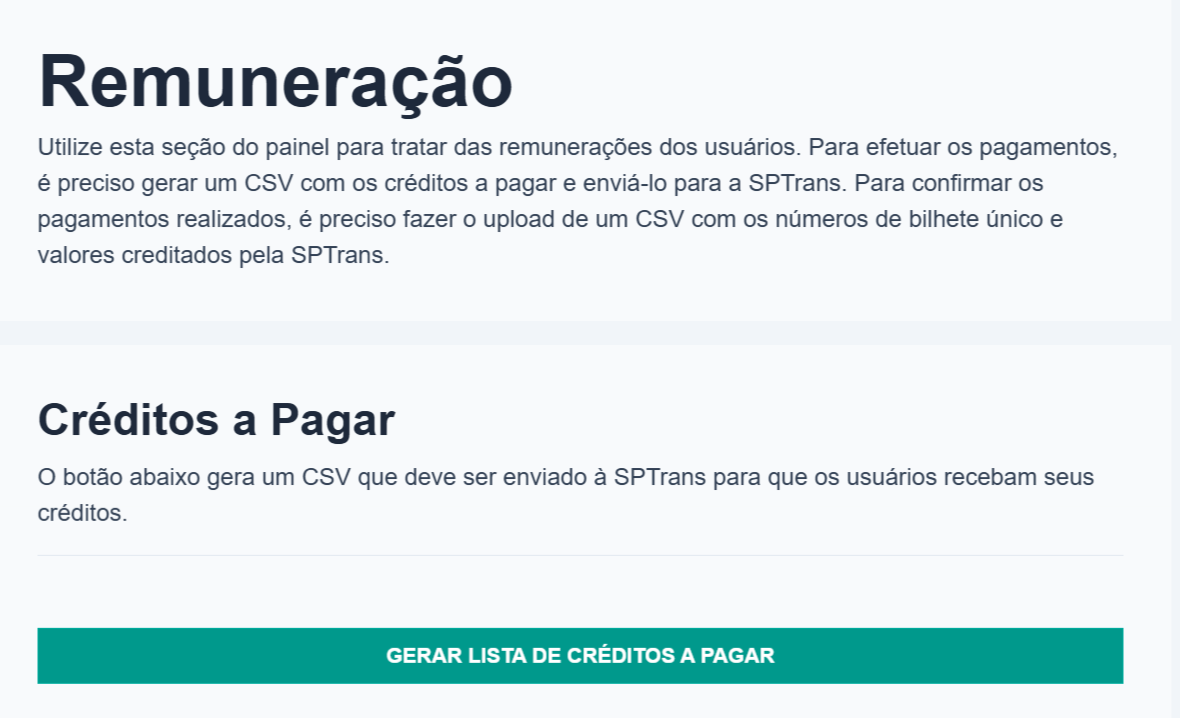
\includegraphics[width=0.95\textwidth]{figuras/remuneracao_creditos.png}
    \caption{Interface de geração de lista de créditos a pagar via SPTrans.}
    \label{fig:remuneracao_gerar_csv_form_creditos}
  \end{figure}

O arquivo CSV gerado é enviado
manualmente à SPTrans. A SPTrans credita os valores nos cartões Bilhete
Único dos participantes e retorna um arquivo CSV de comprovação contendo os bilhetes
efetivamente creditados e os valores pagos. Este processo manual, embora não
automatizado, mostrou-se adequado para a escala do piloto (cerca de 1.200
participantes) e garante supervisão humana sobre transações financeiras, reduzindo
riscos de erros sistêmicos em larga escala.



Ao receber o comprovante da SPTrans,
o administrador realiza upload do arquivo CSV no painel. O sistema executa validação
rigorosa linha por linha: verifica formato (exatas duas colunas), existência do
Bilhete Único no banco de dados, e validade numérica do valor. Qualquer erro
detectado aborta imediatamente o processamento completo, impedindo confirmações
parciais que poderiam gerar inconsistências. Apenas quando todas as linhas são
validadas com sucesso, o sistema processa a confirmação: move valores de
``aguardando resposta'' para ``concedido'', registra o histórico de pagamento como confirmado, e armazena a data e valor de cada operação. Mensagens específicas de erro (``Arquivo com
mais de duas colunas'', ``Formato incorreto de valor'', ``Bilhete não encontrado'')
facilitam correção rápida de problemas antes de reprocessar. A Figura~\ref{fig:remuneracao_gerar_csv_form_processados} ilustra a interface de upload.

\begin{figure}[H]
    \centering
    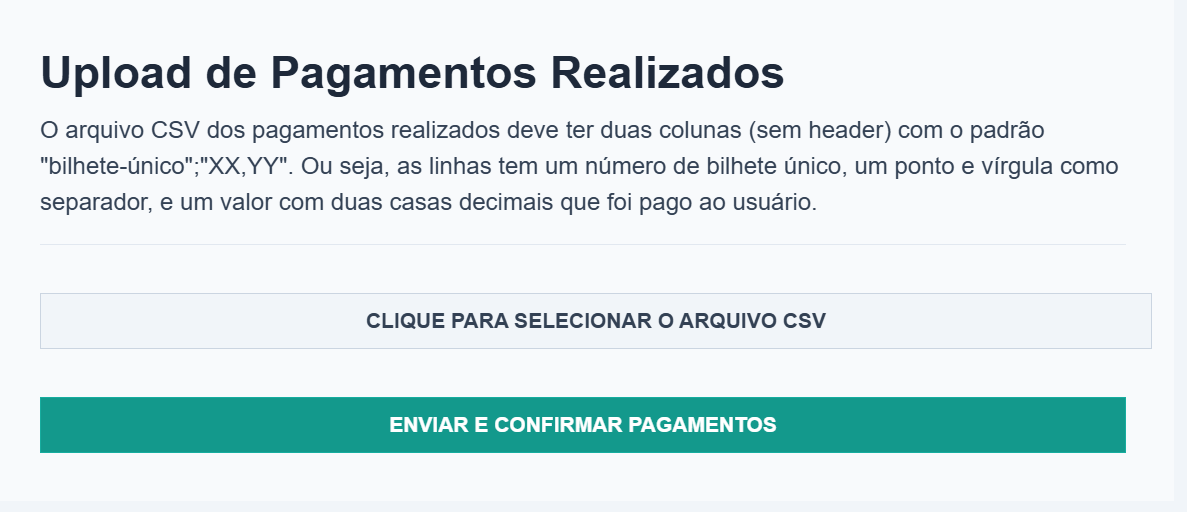
\includegraphics[width=0.95\textwidth]{figuras/remuneracao_processados.png}
    \caption{Interface de upload de comprovante de pagamentos realizados pela SPTrans.}
    \label{fig:remuneracao_gerar_csv_form_processados}
  \end{figure}
O sistema armazena, para cada Bilhete Único, os três estados de remuneração (concedido, aguardando envio, aguardando resposta) além da identificação do participante e status de ativação do cartão. Mantém também registro imutável de todos os envios de pagamento (identificados por número do bilhete e data), permitindo múltiplos pagamentos ao mesmo participante ao longo do tempo. Restrições do banco de dados garantem que valores sejam sempre não
negativos e que transições de estado sigam apenas fluxos
válidos. Toda operação financeira é registrada em log incluindo ID do administrador
responsável, garantindo trilha de auditoria completa e rastreabilidade para
conformidade com procedimentos do experimento.

O painel oferece visibilidade
sobre valores pendentes de envio, valores aguardando confirmação da SPTrans, e total pago aos participantes. 
Durante o piloto, estes indicadores foram fundamentais para
planejamento de fluxo de caixa e comunicação com participantes sobre prazos
esperados de creditação. 

O sistema contempla cenários
atípicos que ocorreram durante operação: (i) pagamentos parciais, quando SPTrans
credita valor inferior ao solicitado, mantendo diferença pendente de confirmação para reenvio posterior; (ii) bilhetes inválidos ou
bloqueados, que não aparecem no CSV de retorno da SPTrans e requerem investigação
manual com o participante; (iii) múltiplos pagamentos no mesmo dia, permitidos via
timestamp distinto na chave primária; e (iv) valores zerados no CSV, que são
ignorados sem gerar erro. A natureza atômica e idempotente do processamento de
confirmações permite reprocessar o mesmo CSV sem duplicações, útil em casos de
falhas de comunicação ou necessidade de revalidação.





\subsection{Contestações}
\label{sec:contestacoes}
%!TeX root=../tese.tex
%("dica" para o editor de texto: este arquivo é parte de um documento maior)

% Conteúdo da subseção sobre Contestações
% Este arquivo é importado em 02-implementacao.tex

O algoritmo de validação automática de viagens implementado no backend Flask rejeitava viagens que não atendiam critérios predefinidos: distância < 1km (consideradas muito curtas para deslocamento cotidiano), origem ou destino fora das localizações cadastradas (potencial fraude ou uso recreacional não remunerável), ou trajetória implausível (teletransportes indicando falha de GPS). Embora estes critérios reduzissem tentativas de fraude, geravam falsos positivos: viagem legítima rejeitada por erro temporário de GPS, localização ligeiramente deslocada devido a imprecisão de geocodificação, ou participante que iniciou pedalada próximo mas não exatamente na localização cadastrada. Sistema de contestações oferece canal para reverter rejeições injustas, balanceando a eficiência da automação com a supervisão humana.

No aplicativo móvel, participantes cujas viagens foram reprovadas visualizam botão ``Contestar'' na tela de detalhes da viagem. Ao clicar, preenchem campo de justificativa explicando por que consideram a viagem válida (ex: ``Saí de casa normalmente, mas GPS demorou para conectar'', ``Trabalho fica dentro de prédio comercial, endereço cadastrado é da entrada principal''). A contestação é enviada e cria registro com status pendente de análise, visível imediatamente na interface administrativa.

A tela administrativa de contestações exibe tabela paginada com ID da pessoa, ID da viagem, data, justificativa, e status (Pendente/Sim/Não). Busca textual cobre todos campos, útil para localizar contestações de participante específico (``busca: 123'') ou por palavra-chave na justificativa (``busca: GPS''). Ao clicar em linha, sistema destaca visualmente e carrega detalhes completos abaixo da tabela, incluindo nome do participante, justificativa integral, e mapa interativo renderizando trajeto GPS da viagem contestada. Visualização do trajeto revelou-se decisória: administrador constata se rota realmente conecta origem-destino, se passou por vias cicláveis, ou se apresenta anomalias (ex: linha reta implausível indicando falha de GPS). A visualização dos trajetos será melhor descrita na seção viagens. A Figura~\ref{fig:contestacoes_listagem} mostra a interface de listagem (dados fictícios para fins ilustrativos).

 \begin{figure}[H]
   \centering
   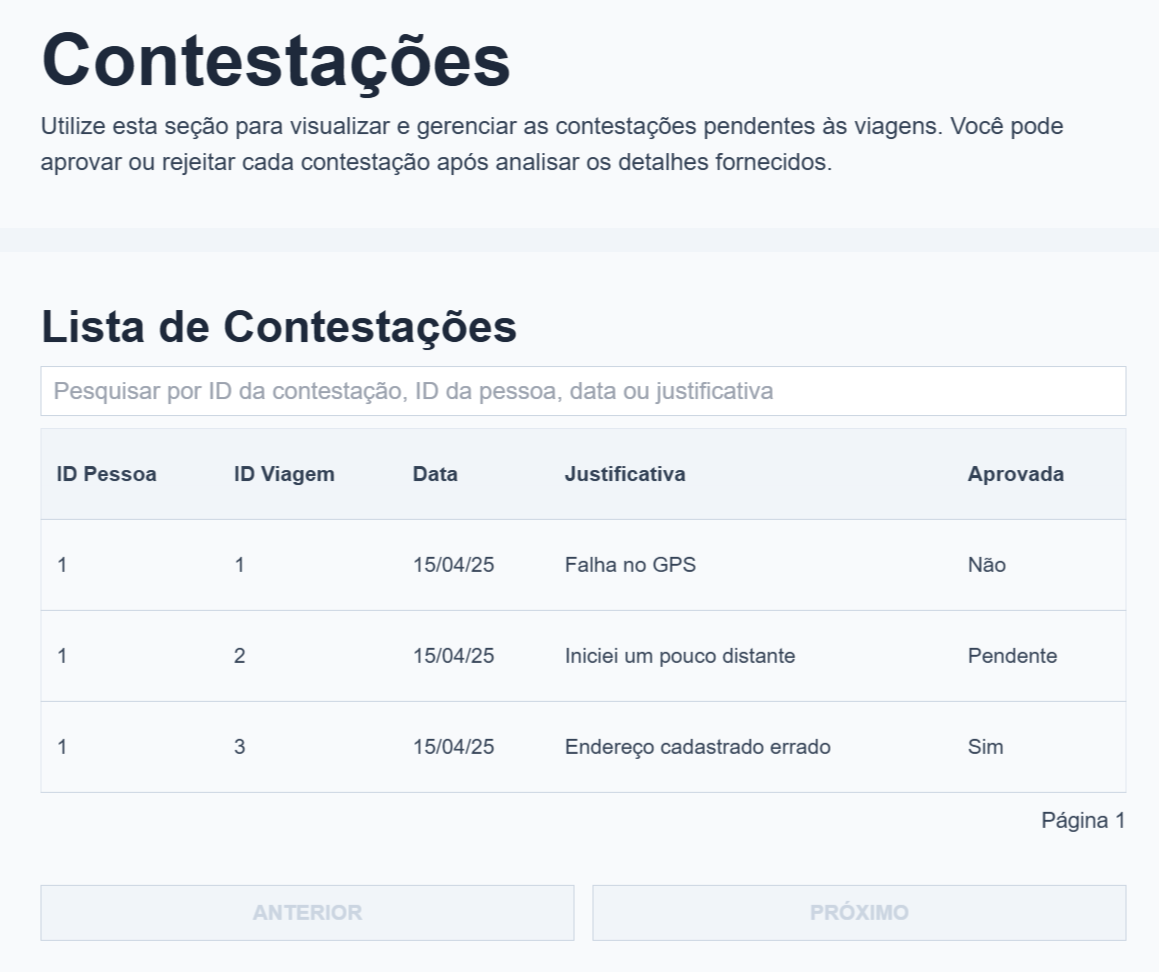
\includegraphics[width=0.95\textwidth]{figuras/contestacoes_listar.png}
   \caption{Interface de listagem de contestações com busca e paginação (dados fictícios).}
   \label{fig:contestacoes_listagem}
 \end{figure}



Após analisar mapa e justificativa, administrador pode aprovar contestação clicando botão com confirmação de duplo clique (prevenção contra aprovação acidental). Sistema executa validações adicionais: contestação não pode ter sido processada anteriormente, viagem deve ter origem e destino definidos e distintos, usuário deve estar em coorte ativa, e distância entre origem-destino $\geq$ 1km. Cálculo de remuneração segue fórmula oficial: \texttt{distancia\_km = min(8000, distancia\_metros) / 1000; remuneracao = distancia\_km * valor\_por\_km\_da\_coorte}. Distância é limitada em 8km (viagens mais longas recebem teto de 8km) para controlar orçamento. Ao aprovar, sistema: atualiza status da viagem para ``Aprovado'', salva valor de remuneração, adiciona crédito à fila de pagamentos, marca a contestação como aprovada, e opcionalmente salva resposta textual do administrador (feedback ao participante). Mensagem de sucesso confirma: ``Contestação da viagem 12345 aprovada com remuneração de R\$ 4,50''. A Figura~\ref{fig:contestacao_aprovar} ilustra a interface de aprovação/rejeição (dados fictícios para fins ilustrativos).

 
\begin{figure}[H]
    \centering
    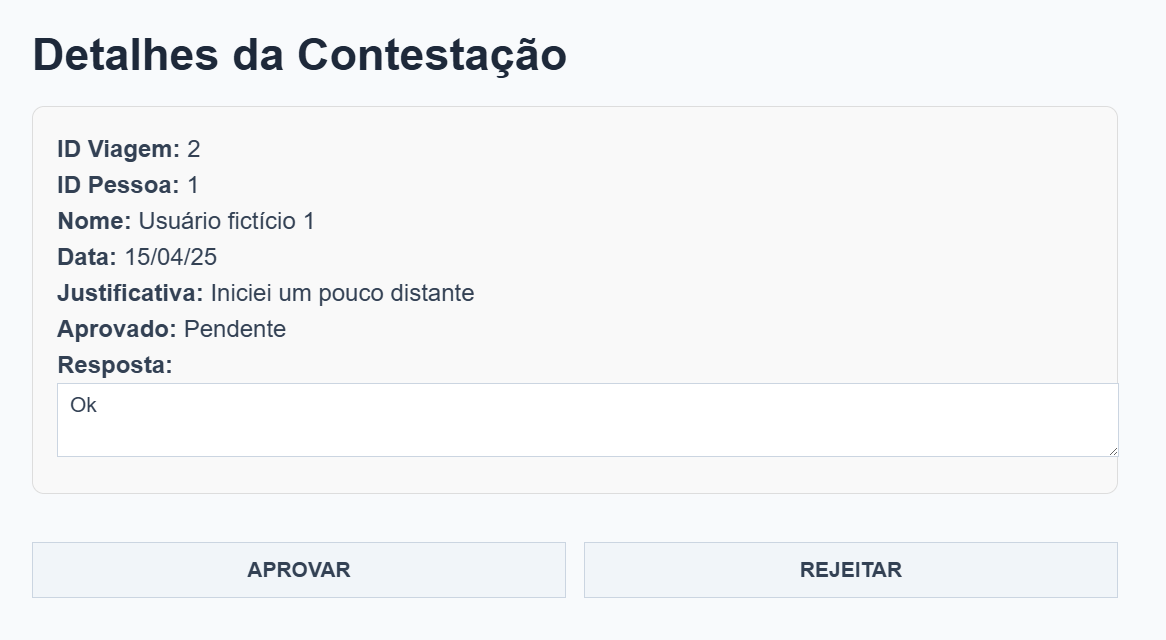
\includegraphics[width=0.95\textwidth]{figuras/contestacao_aprovar.PNG}
    \caption{Interface de aprovação/rejeição de contestação (dados fictícios).}
    \label{fig:contestacao_aprovar}
  \end{figure}

O administrador pode rejeitar contestação (também com confirmação dupla) quando: trajeto não conecta localizações cadastradas (participante tentou viagem recreacional), distância insuficiente mesmo com tolerância, ou justificativa indica má-fé (``não sabia que precisava ativar GPS''). Sistema atualiza contestação para reprovada, salva resposta opcional explicando motivo da rejeição (ex: ``Trajeto iniciou 2km distante da localização cadastrada. Por favor, inicie viagens próximo aos endereços registrados.''), e mantém viagem com status reprovado original. Campo de resposta é exibido no aplicativo móvel, permitindo participante compreender razão e ajustar comportamento futuro.

O sistema implementa múltiplas validações com mensagens específicas orientando correção: ``CONTESTAÇÃO INVÁLIDA'' (ID não encontrado), ``CONTESTAÇÃO JÁ GERENCIADA'' (processamento duplicado prevenido), ``VALOR FALTANDO PARA VIAGEM COM ORIGEM OU DESTINO DESCONHECIDO'' (dados incompletos na viagem), ``VALOR FALTANDO PARA VIAGEM COM ORIGEM == DESTINO'' (mesmo local), ``PESSOA SEM GRUPO PESQUISA'' (usuário não atribuído a coorte), ``DISTANCIA MENOR QUE 1KM'' (critério mínimo não atendido). Estas mensagens, além de prevenir estados inconsistentes no banco de dados, comunicam ao administrador qual condição falhou, permitindo diagnóstico e correção manual (ex: atribuir usuário a coorte antes de reaprovar contestação).



\subsection{Viagens}
\label{sec:viagens}
%!TeX root=../tese.tex
%("dica" para o editor de texto: este arquivo é parte de um documento maior)

% Conteúdo da subseção sobre Viagens
% Este arquivo é importado em 02-implementacao.tex

Durante os seis meses do piloto BikeSP, foram registradas mais de 29.000 viagens pelo aplicativo Android dos participantes, totalizando mais de 150.000 km pedalados. Este volume de dados demandou interface robusta para visualização, busca e análise pela equipe de suporte e pesquisadores. A tela de viagens tornou-se ferramenta essencial para diagnóstico de problemas reportados por usuários (``minha viagem não apareceu'', ``valor creditado está incorreto''), validação de contestações, e análises exploratórias para publicações científicas.

A tabela de viagens apresenta oito colunas principais: ID da viagem (identificador único), ID do usuário, data da viagem, deslocamento em metros, IDs de origem e destino (referenciando localizações cadastradas), status (aprovada/reprovada), e remuneração calculada em reais. O sistema consulta dados de viagens vinculando informações de pessoas e localizações de origem e destino, utilizando técnicas de paginação eficiente para responsividade. Ordenação padrão por ID decrescente exibe viagens mais recentes primeiro, padrão adequado para monitoramento operacional diário.

O campo de busca permite filtrar viagens por ID de usuário específico (busca exata). Esta funcionalidade atende cenário operacional frequente: participante relata problema com viagem; administrador identifica ID do usuário na tela de participantes; busca todas viagens daquele usuário; localiza a viagem em questão (geralmente reconhecível por data/horário ou trajeto).

 \begin{figure}[H]
   \centering
   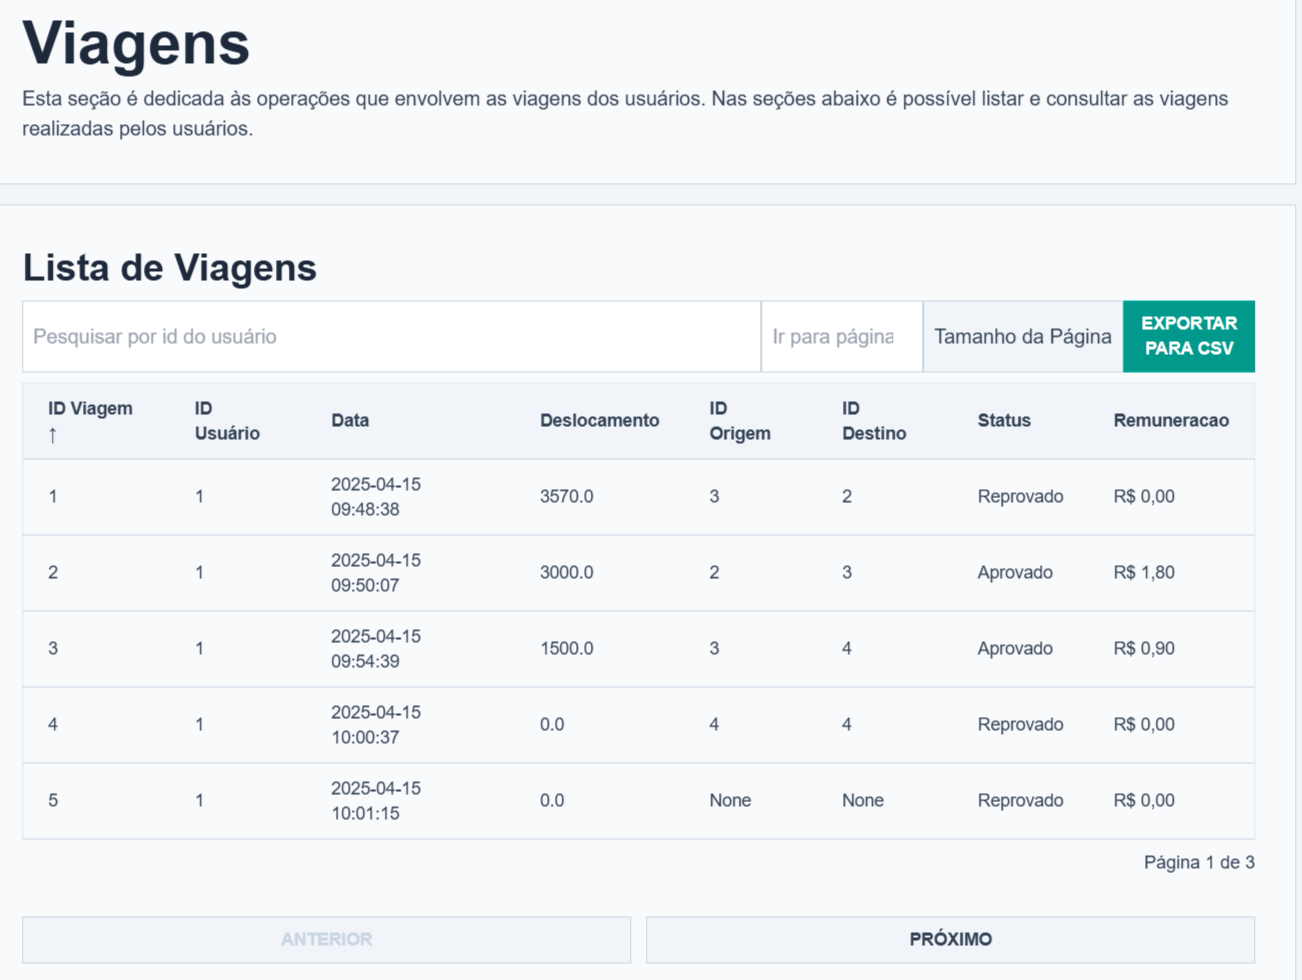
\includegraphics[width=0.95\textwidth]{figuras/viagens_listar.png}
   \caption{Interface de listagem de viagens com funcionalidades de busca, ordenação e paginação.}
   \label{fig:viagens_listar}
 \end{figure}

Ao clicar em qualquer linha da tabela, a interface renderiza mapa interativo (biblioteca Leaflet.js com tiles OpenStreetMap) exibindo trajeto completo da viagem abaixo da tabela. O mapa plota marcadores para cada ponto GPS coletado pelo aplicativo durante a viagem, conectados por linha azul na ordem temporal. Popups nos marcadores exibem timestamp de cada ponto. Zoom automático enquadra toda rota, e controles padrão (zoom, pan, scroll) permitem inspeção detalhada. Esta funcionalidade revelou-se crítica para validação de viagens contestadas: administradores visualizavam se trajeto realmente conectava origem e destino declarados, se passava por vias adequadas para ciclismo, e se não apresentava anomalias (ex: teletransportes indicando GPS incorreto).

\begin{figure}[H]
    \centering
    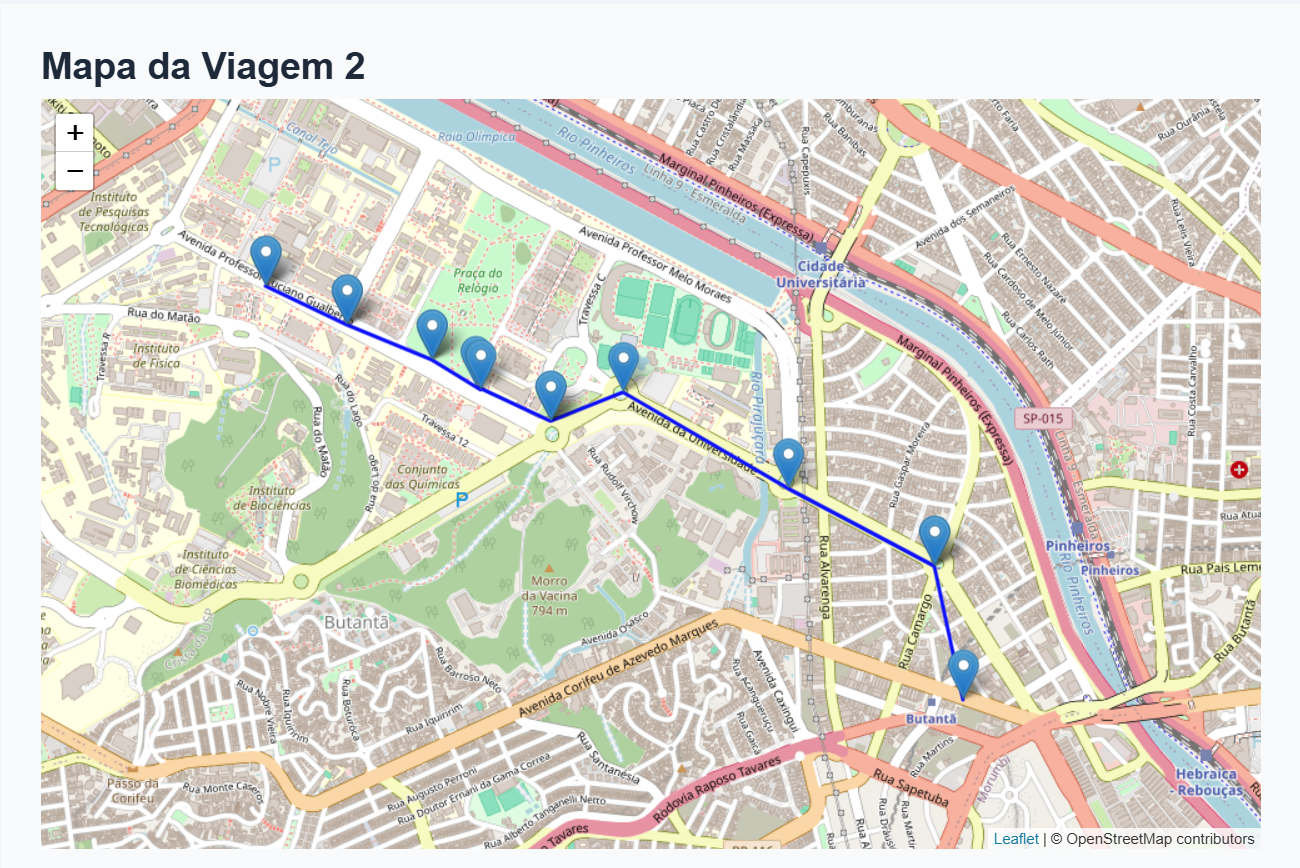
\includegraphics[width=0.95\textwidth]{figuras/mapa_contestacao.PNG}
    \caption{Visualização de trajeto de viagem fictícia com origem no IME e destino na estação Butantã no mapa interativo com marcadores de pontos GPS.}
    \label{fig:mapa_contestacao}
  \end{figure}

O botão de exportação gera arquivo CSV contendo todas as informações exibidas (respeitando filtros de busca ativos) para análise em ferramentas externas. O formato inclui cabeçalho descritivo e delimitador ponto-e-vírgula. Durante piloto, esta funcionalidade foi utilizada semanalmente por economistas do projeto para análises estatísticas: modelos de regressão investigando impacto das coortes no número de viagens, análises de série temporal identificando padrões de uso ao longo da semana, e visualizações geoespaciais em GIS identificando origens/destinos mais frequentes. A possibilidade de exportar dados filtrados (ex: apenas viagens de determinado usuário ou período) reduziu necessidade de consultas diretas ao banco de dados para análises.

A ordenação por diferentes colunas viabiliza análises rápidas: ordenar por deslocamento descendente identifica viagens mais longas (útil para identificar outliers ou comportamento atípico); ordenar por data permite inspeção cronológica (verificar se sistema registrou viagens durante manutenções); ordenar por status agrupa aprovadas vs. reprovadas (calcular taxa de aprovação manual); ordenar por remuneração identifica viagens de maior valor. Durante análise dos resultados do piloto, observou-se que 9 das 10 viagens mais longas (identificadas via ordenação por deslocamento) ocorreram em finais de semana sem remuneração, evidência importante de retenção intrínseca do hábito de pedalar para além do incentivo financeiro.

A configuração padrão de 10 viagens por página balanceia densidade de informação e tempo de carregamento. Com 29.000+ registros, carregar todas viagens simultaneamente seria inviável; paginação server-side (LIMIT/OFFSET no PostgreSQL) mantém responsividade independente do volume total. Indicador ``Página X de Y'' fornece senso de escala, reforçando necessidade de busca e ordenação para localizar informação relevante. Opções de 5, 15 ou 20 itens por página atendem diferentes casos de uso: densidade baixa para inspeção cuidadosa com múltiplos mapas abertos; densidade alta para varredura rápida de padrões.

\textit{Cenário 1: Diagnóstico de viagem não creditada} --- participante relata viagem realizada ontem não apareceu no extrato; administrador busca por ID do usuário, filtra viagens recentes (ordenação por data), identifica viagem com status ``reprovada''; visualiza mapa, constata que trajeto passou por localizações não cadastradas; orienta participante a atualizar endereços. \textit{Cenário 2: Validação de contestação} --- usuário contesta rejeição de viagem; administrador abre viagem contestada, visualiza mapa, confirma que trajeto conecta origem e destino cadastrados; aprova contestação, gerando remuneração retroativa.




\subsection{Notificações}
\label{sec:notificacoes}
%!TeX root=../Monografia - Mikhael Pinto.tex
%("dica" para o editor de texto: este arquivo é parte de um documento maior)

% Conteúdo da subseção sobre Notificações
% Este arquivo é importado em 02-implementacao.tex

%acho que teve comunicação nas coortes%
Com 1.217 participantes distribuídos geograficamente por São Paulo e engajados em experimento com rotação semanal de coortes, estabelecer canal eficaz de comunicação mostrou-se crítico. Eventos requerendo notificação incluíam: início de nova coorte (informar mudança de remuneração), disponibilidade de pagamento (créditos depositados no Bilhete Único), manutenções programadas no sistema, lembretes de preenchimento de questionários qualitativos, e esclarecimentos sobre regras do experimento após dúvidas recorrentes. Sistema de notificações implementado no painel oferece dois canais simultâneos: push notifications via Firebase Cloud Messaging (FCM) para aplicativo Android, e email via SMTP (Gmail) para endereços cadastrados.

A interface oferece três estratégias de direcionamento: (i) envio individual para IDs específicos separados por vírgula (ex: comunicação de suporte técnico, ``participantes 123, 456 e 789: problema reportado foi corrigido''); (ii) envio por coorte via IDs de grupos experimentais (ex: ``participantes da coorte 2: esta semana sua remuneração é R\$~0,60/km''); e (iii) broadcast para todos participantes cadastrados (ex: ``sistema em manutenção dia 15 das 02h-04h''). Esta granularidade atende necessidades distintas: comunicação individualizada reduz ruído para participantes não afetados; segmentação por coorte mantém integridade do desenho experimental (evitando confusão sobre qual valor de remuneração aplica-se a cada grupo); broadcast garante que informações críticas alcancem todos.

O formulário de criação requer título (usado como assunto de email e cabeçalho de push notification) e corpo da mensagem. Campo de corpo aceita HTML completo, permitindo formatação rica em emails: parágrafos (\texttt{<p>}), quebras de linha (\texttt{<br>}), negrito (\texttt{<strong>}), listas, e links. Suporte a HTML mostrou-se valioso para comunicações longas ou complexas, como FAQ respondendo dúvidas recorrentes ou instruções passo-a-passo para resolver problemas comuns. Push notifications, devido a limitações de espaço em dispositivos móveis, exibem apenas texto plano, adequado para mensagens concisas. Checkbox independentes para cada canal (push e/ou email) permitem escolher meio mais apropriado: push para alertas urgentes que requerem atenção imediata; email para informações detalhadas que usuário pode consultar posteriormente. A Figura~\ref{fig:notificacao_criar} mostra a interface de criação.

 \begin{figure}[htb]
   \centering
   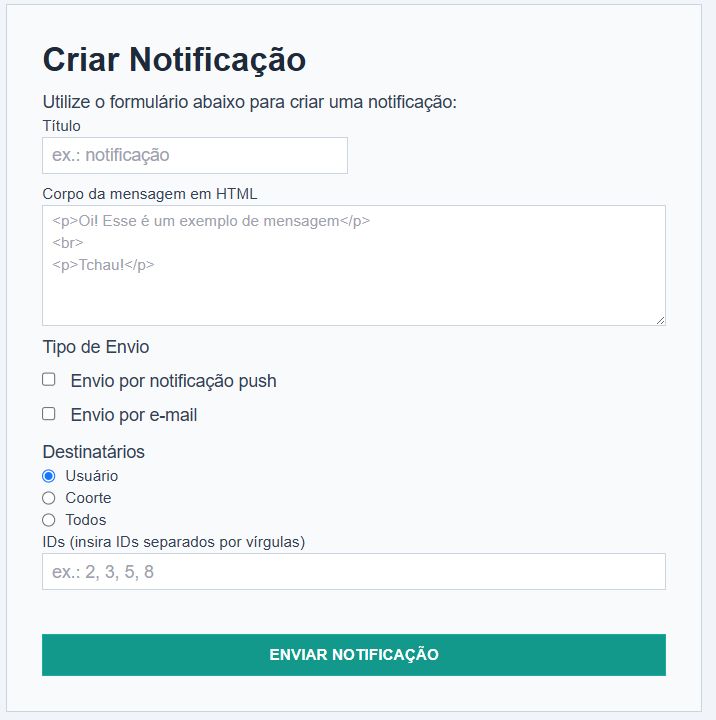
\includegraphics[width=0.95\textwidth]{figuras/notificacao_criar.PNG}
   \caption{Formulário de criação e envio de notificações para participantes.}
   \label{fig:notificacao_criar}
 \end{figure}

Para push notifications, o sistema consulta tabela de tokens FCM associados a cada participante (registrados durante primeira abertura do aplicativo), envia payload via API do Firebase, e notificação aparece na bandeja de notificações Android do participante. Falhas ocasionais ocorrem quando aplicativo é desinstalado ou token expira. Para emails, sistema busca endereços cadastrados, envia via protocolo SMTP autenticado em conta Gmail institucional, posicionando destinatários em BCC (cópia oculta para privacidade) e destinatário padrão configurável (tipicamente \texttt{bikesp-app@ime.usp.br}) no campo ``Para''. Esta arquitetura preserva privacidade (nenhum participante vê emails de outros) e profissionalismo (remetente institucional aumenta confiabilidade, reduzindo classificação como spam).

A funcionalidade de cópia oculta para email do administrador que enviou a notificação (mencionada em documentação como ``enviadas em cópia oculta para o email do administrador'') cria trilha de auditoria e permite verificação imediata de conteúdo e destinatários. Este registro mostrou-se útil para resolver disputas e manter histórico de comunicações para análise de engajamento.

O sistema valida que ao menos um canal (push ou email) está selecionado; que IDs de usuários/coortes são numéricos; e que campo de IDs é obrigatório apenas quando estratégia ``Usuário'' ou ``Coorte'' está selecionada (e escondida quando ``Todos'' marcado). Log de todas operações registra quem enviou, para quem, quando, e conteúdo da mensagem.

O sistema de notificações foi utilizado para diversos fins: broadcasts (anúncios gerais, disponibilidade de pagamentos), notificações por coorte (lembretes de remuneração ativa, instruções específicas), e mensagens individuais (suporte técnico, correções de problemas).




\subsection{Localizações}
\label{sec:localizacoes}
%!TeX root=../Monografia - Mikhael Pinto.tex
%("dica" para o editor de texto: este arquivo é parte de um documento maior)

% Conteúdo da subseção sobre Localizações
% Este arquivo é importado em 02-implementacao.tex

O desenho do experimento BikeSP especificou que apenas viagens entre localizações pré-cadastradas seriam remuneradas, visando incentivar deslocamentos cotidianos (casa-trabalho, casa-escola) em detrimento de viagens recreacionais irregulares. Durante inscrição via formulário LimeSurvey, participantes forneciam endereços textuais de até três localizações principais (tipicamente residência, trabalho/estudo, e uma terceira opcional). O sistema realizava geocodificação automática destes endereços  --- conversão de texto (``Av. Paulista, 1000, Bela Vista, CEP 01310-100'') para coordenadas GPS (latitude/longitude) utilizando APIs externas de geolocalização.

Para prevenir fraudes (participante alterando localizações para simular viagens longas fictícias), implementou-se regra de uma única alteração por localização após cadastro inicial. Participante que cadastrasse endereço incorreto ou mudasse de residência/trabalho poderia corrigi-lo uma vez via aplicativo; segunda tentativa de alteração seria bloqueada. Esta restrição, embora necessária para integridade experimental, gerou demandas de suporte quando usuários cometiam erros tipográficos ou mudavam endereço legitimamente após já terem usado sua cota de alteração.

A interface administrativa de localizações permite buscar por ID de participante e visualizar todas localizações cadastradas (ID, endereço completo, coordenadas, tipo). Funcionalidade crítica é reset da permissão de alteração: administrador, após validar legitimidade da solicitação via email ou telefone, pode remover o registro que controla alterações de localização, concedendo ao participante nova oportunidade de modificar endereço no aplicativo. Mensagens de feedback (``O usuário agora pode trocar uma localização'' vs. ``Nenhuma alteração de localização foi encontrada'') informam sucesso ou ausência de restrição ativa. Este procedimento foi utilizado durante o piloto, geralmente após mudanças residenciais ou correções de erros de digitação durante inscrição inicial.

Durante o script de inserção em lote de participantes do LimeSurvey para PostgreSQL, alguns endereços falhavam em geocodificação automática. Causas possíveis incluíam: formatação inconsistente (``Rua X, 100'' vs. ``Rua X|100|...''), abreviações não reconhecidas, bairros incorretos, CEPs inválidos, endereços recém-criados ausentes em bases cartográficas, e timeouts de APIs. Localizações que falhavam geocodificação eram marcadas como ``inválidas'' e ficavam inacessíveis no aplicativo móvel ---  participante visualizava localização na lista mas não podia utilizá-la como origem/destino de viagens, bloqueando efetivamente sua participação.

Este problema revelou-se crítico: correção manual urgente foi necessária durante o piloto. A funcionalidade de correção de geolocalização tornou-se operação essencial.

A tela de localizações inválidas lista endereços que falharam, exibindo ID, ID do participante, endereço textual, tipo e apelido da localização. Funcionalidades de busca, ordenação e paginação seguem padrão estabelecido em outras telas. Para corrigir, administrador edita endereço diretamente seguindo dois formatos possíveis: (i) endereço estruturado separado por pipe (ex: \texttt{Av. Paulista|1000|sala 5|Bela Vista|01310-100|São Paulo|SP}), submetido novamente às APIs de geocodificação; ou (ii) coordenadas GPS diretas (ex: \texttt{-23.5997136,-46.4677964}), sem precisar passar pela geocodificação quando endereço é intratável por APIs mas localização é conhecida via Google Maps. Validação bem-sucedida remove localização da lista de inválidas, tornando-a imediatamente disponível no aplicativo do participante.

Workflow operacional típico incluía: cópia do endereço para Google Maps, verificação de formatação e bairro correto, ajuste se necessário, validação no sistema. Problemas recorrentes e soluções documentadas: CEPs com dígitos transpostos (buscar CEP correto online); bairros coloquiais vs. oficiais (Pinheiros vs. Alto de Pinheiros); abreviações (``Av.'' expandir para ``Avenida''); endereços inexistentes (usar coordenadas GPS obtidas manualmente). A disponibilidade de múltiplas APIs de geolocalização aumentava taxa de sucesso, mas timeouts ocasionais justificavam opção de inserção direta de coordenadas.

A correção de localizações inválidas foi realizada pela equipe de suporte. Diferentes abordagens foram utilizadas: reformatação com nova geocodificação automática, inserção manual de coordenadas diretas obtidas via Google Maps, ou contato com participante para clarificação de endereço.

Para iterações futuras do programa, recomendações incluem: validação de formato durante preenchimento do formulário LimeSurvey, geocodificação imediata após submissão do formulário com feedback visual ao candidato, e assistente de endereçamento integrado (autocompletar baseado em API de CEPs). A natureza manual e laboriosa da correção em lote demonstrou ser gargalo operacional não escalável: expansão para 10.000 participantes (meta de implementação municipal completa) seria inviável sem automação adicional nesta etapa.




Após a descrição detalhada da implementação do painel administrativo e suas funcionalidades, o próximo capítulo apresenta os resultados alcançados durante a execução do piloto, incluindo dados quantitativos de uso e uma avaliação do impacto do sistema nas operações.

